\documentclass{article}
\iffalse
This file is protected by Copyright. Please refer to the COPYRIGHT file
distributed with this source distribution.

This file is part of OpenCPI <http://www.opencpi.org>

OpenCPI is free software: you can redistribute it and/or modify it under the
terms of the GNU Lesser General Public License as published by the Free Software
Foundation, either version 3 of the License, or (at your option) any later
version.

OpenCPI is distributed in the hope that it will be useful, but WITHOUT ANY
WARRANTY; without even the implied warranty of MERCHANTABILITY or FITNESS FOR A
PARTICULAR PURPOSE. See the GNU Lesser General Public License for more details.

You should have received a copy of the GNU Lesser General Public License along
with this program. If not, see <http://www.gnu.org/licenses/>.
\fi

\author{} % Force author to be blank
%----------------------------------------------------------------------------------------
% Paper size, orientation and margins
%----------------------------------------------------------------------------------------
\usepackage{geometry}
\geometry{
  letterpaper,      % paper type
  portrait,       % text direction
  left=.75in,       % left margin
  top=.75in,        % top margin
  right=.75in,      % right margin
  bottom=.75in      % bottom margin
 }
%----------------------------------------------------------------------------------------
% Header/Footer
%----------------------------------------------------------------------------------------
\usepackage{fancyhdr} \pagestyle{fancy} % required for fancy headers
\renewcommand{\headrulewidth}{0.5pt}
\renewcommand{\footrulewidth}{0.5pt}
\newcommand{\terminaloutput}[1]{\texttt{#1}}
\rhead{\small{ANGRYVIPER Team}}
%----------------------------------------------------------------------------------------
% Appendix packages
%----------------------------------------------------------------------------------------
\usepackage[toc,page]{appendix}
%----------------------------------------------------------------------------------------
% Defined Commands & Renamed Commands
%----------------------------------------------------------------------------------------
\renewcommand{\contentsname}{Table of Contents}
\renewcommand{\listfigurename}{List of Figures}
\renewcommand{\listtablename}{List of Tables}
\newcommand{\todo}[1]{\textcolor{red}{TODO: #1}\PackageWarning{TODO:}{#1}} % To do notes
\newcommand{\code}[1]{\texttt{#1}} % For inline code snippet or command line
%----------------------------------------------------------------------------------------
% Various pacakges
%----------------------------------------------------------------------------------------
\usepackage{hyperref} % for linking urls and lists
\usepackage{graphicx} % for including pictures by file
\usepackage{listings} % for coding language styles
\usepackage{rotating} % for sideways table
\usepackage{pifont}   % for sideways table
\usepackage{pdflscape} % for landscape view
\usepackage{longtable}
%----------------------------------------------------------------------------------------
% Table packages
%----------------------------------------------------------------------------------------
\usepackage{tabularx} % c=center,l=left,r=right,X=fill
\usepackage{float}
\floatstyle{plaintop}
\usepackage[tableposition=top]{caption}
\newcolumntype{P}[1]{>{\centering\arraybackslash}p{#1}}
\newcolumntype{M}[1]{>{\centering\arraybackslash}m{#1}}
%----------------------------------------------------------------------------------------
% Block Diagram / FSM Drawings
%----------------------------------------------------------------------------------------
\usepackage{tikz}
\usetikzlibrary{shapes,arrows,fit,positioning}
\usetikzlibrary{automata} % used for the fsm
\usetikzlibrary{calc} % For duplicating clients
\usepgfmodule{oo} % To define a client box
%----------------------------------------------------------------------------------------
% Colors Used
%----------------------------------------------------------------------------------------
\usepackage{colortbl}
\definecolor{blue}{rgb}{.7,.8,.9}
\definecolor{ceruleanblue}{rgb}{0.16, 0.32, 0.75}
\definecolor{drkgreen}{rgb}{0,0.6,0}
\definecolor{deepmagenta}{rgb}{0.8, 0.0, 0.8}
\definecolor{cyan}{rgb}{0.0,0.6,0.6}
\definecolor{maroon}{rgb}{0.5,0,0}
\usepackage{multirow}
%----------------------------------------------------------------------------------------
% Update the docTitle and docVersion per document
%----------------------------------------------------------------------------------------
\def\docTitle{Component Data Sheet}
\def\docVersion{1.3}
%----------------------------------------------------------------------------------------
\date{Version \docVersion} % Force date to be blank and override date with version
\title{\docTitle}
\lhead{\small{\docTitle}}

\def\comp{lime\_tx}
\def\Comp{Lime TX}
\graphicspath{ {figures/} }

\begin{document}

\section*{Summary - \Comp}
\begin{tabular}{|c|M{13.5cm}|}
  \hline
  \rowcolor{blue}
                    &                  \\
  \hline
  Name              & \comp            \\
  \hline
  Worker Type       & Device           \\
  \hline
  Version           & v\docVersion{}   \\
  \hline
  Release Date      & Oct 2017         \\
  \hline
  Component Library & ocpi.devices     \\
  \hline
  Workers           & \comp.hdl        \\
  \hline
  Tested Platforms  & Matchstiq Z1, Zedboard (Vivado), ISIM, MODELSIM, XSIM \\
  \hline
\end{tabular}

\section*{Functionality}
  The \Comp{} is a worker which provides an entry point to the TX functionality of the Lime LMS6002D IC. The worker is a master for the IC's SPI bus for intercommunication with the Lime LMS6002D register map. Note that, while the register address decoding is performed within this worker, the SPI state machine itself is implemented in one or more separate, platform-specific or card-specific subdevice workers.

\section*{Worker Implementation Details}
\subsection*{\comp.hdl}
The Lime LMS6002D register map is realized via a rawprops port whose communication is forwarded on to a SPI subdevice worker. The register map is implemented via the Component Spec properties for this worker, all of which correspond with the Lime LMS6002D register map. This worker also has an input port which can turn on/off the transmitter for support of burst transmit applications.

\section*{Block Diagrams}
\subsection*{Top level}
\begin{center}
	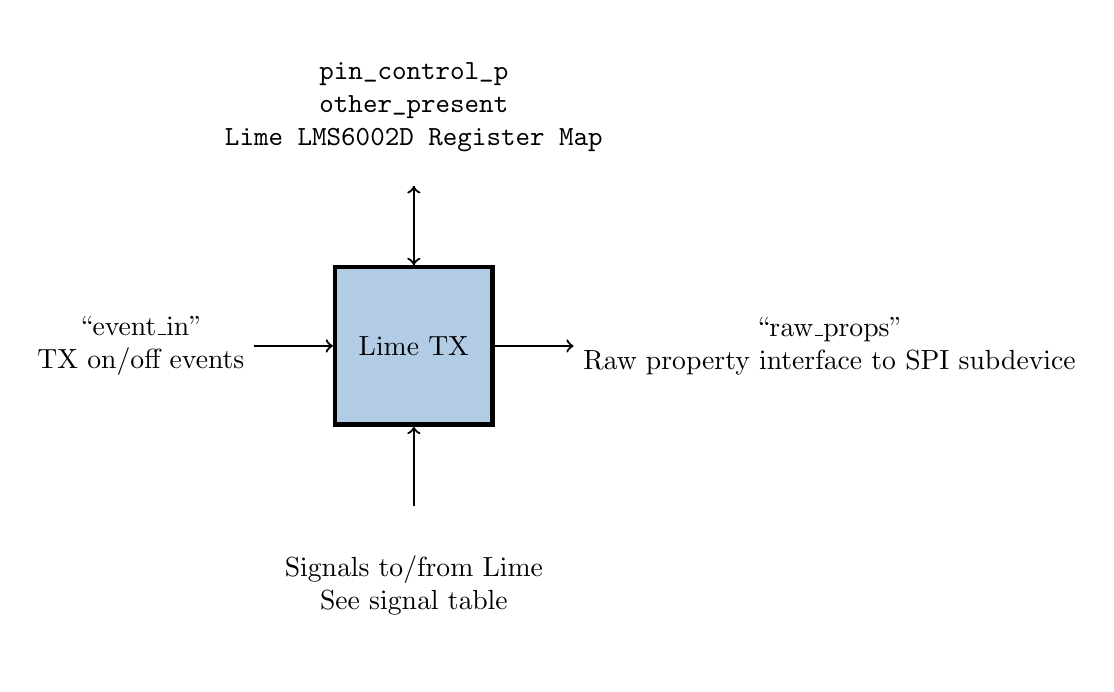
\begin{tikzpicture}[% List of styles applied to all, to override specify on a case-by-case
			every node/.style={
				align=center,  		% use this so that the "\\" for line break works
				minimum size=2cm	% creates space above and below text in rectangle
			},
			every edge/.style={draw,thick}
		]
		\node[rectangle,ultra thick,draw=black,fill=blue](R2){\Comp};
		\node[rectangle,draw=white,fill=white](R3)[below= of R2]{Signals to/from Lime \\ See signal table};
		\node[rectangle,draw=white,fill=white](R4)[left= of R2]{``event\_in'' \\ TX on/off events};
		\node[rectangle,draw=white,fill=white](R5)[above= of R2]{\verb+pin_control_p+\\\verb+other_present+\\\verb+Lime LMS6002D Register Map+};
		\node[rectangle,draw=white,fill=white](R6)[right= of R2]{``raw\_props'' \\ Raw property interface to SPI subdevice};
		\path[->]
		(R3)edge []	node [] {} (R2)
		(R4)edge []	node [] {} (R2)
		(R2)edge []	node [] {} (R5)
		(R5)edge []	node [] {} (R2)
		(R2)edge []	node [] {} (R6)
		;
	\end{tikzpicture}
\end{center}

\section*{Source Dependencies}
\subsection*{\comp.hdl}
\begin{itemize}
  \item opencpi/hdl/devices/\comp{}.hdl/\comp{}.vhd
\end{itemize}
\begin{landscape}

  \section*{Component Spec Properties}
  \begin{scriptsize}
  \subsection*{\comp.hdl}
      \begin{tabular}{|p{2cm}|p{2cm}|p{1cm}|c|c|p{1.75cm}|p{1.5cm}|p{7cm}|}
      \hline
      \rowcolor{blue}
      Scope    & Name  				& Type  & Sequence Length 	& Array Dimensions 	& Accessibility & Valid Range 	& Usage \\
      \hline
      - & - & - & - & - & - & - & - \\
      \hline
  \end{tabular}
  \end{scriptsize}

  \section*{Component Ports}
  \begin{scriptsize}
    \begin{tabular}{|p{2cm}|p{1.5cm}|p{4cm}|p{1.5cm}|p{1.5cm}|p{10.85cm}|}
      \hline
      \rowcolor{blue}
      Name 		& Producer & Protocol           & Optional & Advanced & Usage      		\\
      \hline
      event\_in & -        & tx\_event-prot     & -        & -        & TX on/off events\\
      \hline
    \end{tabular}
  \end{scriptsize}

  \section*{Worker Properties}
  \begin{scriptsize}
    \begin{tabular}{|p{3.75cm}|p{1.25cm}|p{2cm}|p{2.75cm}|p{1.5cm}|p{1.5cm}|p{1cm}|p{6.74cm}|}
      \hline
      \rowcolor{blue}
      Name               & Type & SequenceLength & ArrayDimensions & Accessibility      & Valid Range & Default & Usage                                                                               \\
      \hline
      Property & pin\_control\_p 	& Bool 	& - 				& - 				& Parameter		& Standard 		& TXEN signal is connected to Lime LMS6002D. \\
      \hline
      Property & other\_present 	& Bool 	& - 				& - 				& Readable 		& Standard 		& Value is true if raw property port is connected. \\
      \hline
    \end{tabular}
  \end{scriptsize}

  \section*{Worker Interfaces}
  \subsection*{\comp.hdl}
	\begin{scriptsize}
		\begin{tabular}{|M{2cm}|M{1.5cm}|c|c|M{12cm}|}
			\hline
			\rowcolor{blue}
			Type            & Name 		& DataWidth & Advanced   	& Usage                                    	\\
			\hline
			StreamInterface & event\_in & -        	& optional=true	& TX on/off events							\\
			\hline
			Rawprop 		& rawprops  & -       	& master=true   & Raw property interface to SPI subdevice	\\
			\hline
		\end{tabular}
	\end{scriptsize}

\end{landscape}

\section*{Control Timing and Signals}
The \Comp{} subdevice worker operates in the control plane clock domain. Note that this worker is essentially the central worker that command/control passes through, and no RX or TX data paths flow through this worker.

\begin{landscape}
\section*{Worker Configuration Parameters}
\subsubsection*{\comp.hdl}
\input{../../\ecomp.hdl/configurations.inc}
\section*{Performance and Resource Utilization}
\subsubsection*{\comp.hdl}
\input{../../\ecomp.hdl/utilization.inc}
\end{landscape}

\section*{Test and Verification}
\begin{flushleft}
The unit test for this worker only verifies the event\_in port functionality. It does not verify the SPI functionality of the worker. The test uses a custom Makefile as opposed to the OpenCPI unit test framework.\par\medskip

The test uses another component, test\_tx\_event.hdl, to generate subsequent on and off events and a interval specified via its max\_count\_value property. For simulation, an output file is generated containing either the SPI address/data sent to the subdevice for the pin\_control\_p=false case or the number of on/off events for the pin\_control\_p=true case.\par\medskip

For verification, the output file is compared to a file containing the expected result. For HDL platforms, the test\_tx\_event.hdl worker generates on/off events at 1 second intervals which can be observed on a spectrum analyzer. Response times between the on/off event and transmitter SPI transaction completion for the pin\_control\_p=false case are approximately 5 us. An oscilloscope capture of the response time can be seen in Figure \ref{fig:response_time}
\begin{figure}[ht]
	\centerline{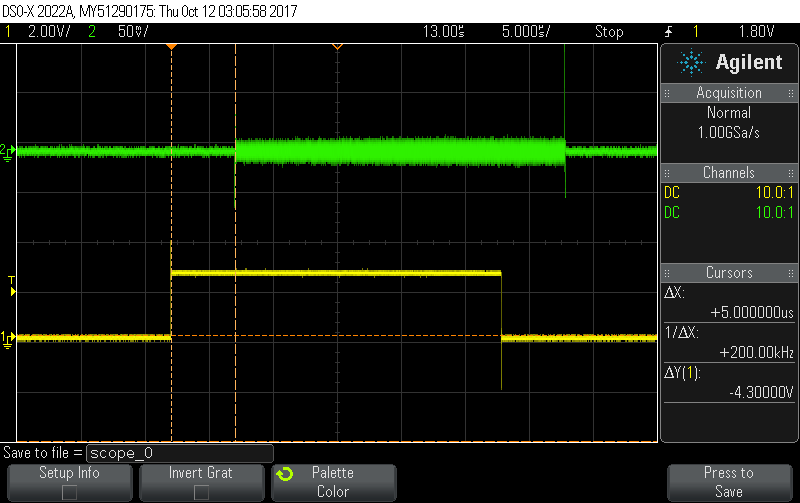
\includegraphics[scale=0.4]{txen_timing_matchstiq_z1}}
	\caption{TX on/off event response time}
	\label{fig:response_time}
\end{figure}
\end{flushleft}
\section*{References}
\begin{itemize}
	\item[1)] LMS6002D Datasheet, www.limemicro.com
\end{itemize}

\end{document}
